\documentclass[a4paper,12pt]{article}

\usepackage[utf8]{inputenc}
\usepackage[T1]{fontenc}
\usepackage[french]{babel}
\usepackage{geometry}
\geometry{a4paper, margin=2cm}
\usepackage{amsmath}
\usepackage{graphicx}
\usepackage{eso-pic}
\usepackage{float}
\usepackage{graphicx}
\usepackage{hyperref}
\usepackage[round]{natbib}
\usepackage{hyperref}
\hypersetup{
    colorlinks=true, 
    linkcolor=black,   
    citecolor=blue,  
    urlcolor=blue    
}
\usepackage{lato}
\renewcommand{\familydefault}{\sfdefault}
\title{Rapport Académique}
\author{Mathys Dussel}
\date{\today}

\usepackage{setspace}

\begin{document}
\singlespacing
\begin{titlepage}
    \centering
    \vspace*{1cm}



\AddToShipoutPictureBG*{
       \AtPageUpperLeft{%
              \put(\LenToUnit{\paperwidth-5cm},\LenToUnit{-2.6cm}){
                     
\includegraphics[width=4.1cm]{Figures/logo-UT.png} 
              }
       }
}
%\AddToShipoutPictureBG*{
       %\AtPageUpperLeft{%
             % \put(\LenToUnit{\paperwidth-9cm},\LenToUnit{-2.8cm}){
                    % 
\includegraphics[width=4cm]{Figures/Logo-CRBE.%png} 
             % }
       %}
%}
\AddToShipoutPictureBG*{
       \AtPageUpperLeft{
              \put(\LenToUnit{\paperwidth-7cm},\LenToUnit{-2.8cm}){
                     
\includegraphics[width=1.4cm]{Figures/LOT.png} 
              }
       }
}
    \vspace{1cm}
    {\scshape\Large Université de Toulouse \par}
    \vspace{1cm}
    
    {\Large\bfseries Stage réalisé dans le cadre du module Initiation à la Recherche \\[0.3cm] Master 1 Biodiversité,
Ecologie et Evolution\par}
    \vspace{0.5cm}
    
    \rule{\linewidth}{0.5mm} \\[0.4cm]
    {\huge \bfseries Composition et assemblage des communautés fongiques chez les plantes épiphytes vasculaires tropicales\par}
    \vspace{0.4cm}
    \rule{\linewidth}{0.5mm} \\[1.5cm]
    

    
    \begin{minipage}{0.4\textwidth}
        \begin{flushleft} \large
            \emph{Étudiant :}\\
            Mathys \textsc{DUSSEL D'HERVÉ}
        \end{flushleft}
    \end{minipage}
    ~
    \begin{minipage}{0.4\textwidth}
        \begin{flushright} \large
            \emph{Tutrice de stage :} \\
            Céline \textsc{Leroy}
        \end{flushright}
    \end{minipage}\\[1cm]
    
    \vfill
    \includegraphics[width=0.65\textwidth]{Figures/branche_chargée.jpeg} % Remplacez par le nom de votre image
    \vfill
    
    {\large Lieu du stage : Centre de Recherche sur la Biodiversité et l'Environnement (CRBE)\par}
     \vfill
    
    {\large Année universitaire 2025-2026\par}
    \vspace{0.5cm}
    {\large \today\par}
\end{titlepage}

\renewcommand{\maketitle}{}
\maketitle

\thispagestyle{empty}
\section*{Avant-propos}
\newpage

\thispagestyle{empty}
\section*{Remerciements}
\newpage


\thispagestyle{empty}
\renewcommand{\contentsname}{\centerline{Sommaire}}
\tableofcontents
\newpage

\setcounter{page}{1}
\section{Résumé}

\textbf{Mots-clés :} Fongique, Epiphyte, Tropical, Diversité, Assemblage, Communauté


\section{Abstract}


\newpage
\onehalfspacing
\section{Introduction}


Les champignons ont une importance cruciale pour le bon fonctionnement des écosystèmes terrestres. Ils animent les cycles biogéochimiques et influencent directement la dynamique des végétaux. Comment ces assemblages microbiens se structurent-ils ? C'est le résultat d'un mélange complexe de facteurs biotiques et abiotiques, comme la température ou l'humidité. Dans les milieux tropicaux, foyers d'une biodiversité record, les liens entre champignons et plantes hôtes prennent une ampleur toute particulière \citep{arnold_are_2000, bermudes_fungi_1989}. Si l'on regarde à l'échelle d'une plante, le microbiote fongique varie beaucoup d'un organe à l'autre (feuilles, racines) et selon son emplacement. On sépare généralement les épiphytes, vivant en surface, des endophytes, présents au cœur des tissus. L'identité de la plante joue un rôle de filtre sélectif. Par ses traits fonctionnels, ses exsudats ou encore son système immunitaire, l'hôte façonne son propre mycobiome.

Afin de mieux saisir ces interactions sous contraintes extrêmes, les plantes épiphytes offrent un modèle d'étude tout trouvé. Elles représentent en effet une part immense de la flore des canopées tropicales et poussent sur d'autres arbres, sans pour autant les parasiter \citep{zotz_plants_2016}. Ce mode de vie « suspendu » les prive d'un accès au sol. Elles subissent un manque d'eau et de nutriments. Pour faire face à ces stress sévères, ces plantes ont dû innover. Elles s'en remettent de manière vitale à des associations avec d'autres organismes : animaux, bactéries ou champignons. Ces alliances mutualistes améliorent leur nutrition et les aident à tenir face au stress ambiant.

Pourtant, malgré un tel enjeu écologique, nos connaissances sur ces communautés fongiques sont encore très légères. Très souvent, la recherche s'est focalisée sur les plantes terrestres. Elle s'est même penchée en priorité sur celles ayant une valeur agronomique sous les tropiques, comme le café ou le cacao \citep{vega_fungal_2008}. Quand on s’intéresse spécifiquement à la flore épiphyte, le constat est similaire : les travaux portent presque toujours sur quelques « stars » écologiques ou économiques. Les \textit{Orchidaceae} en sont le meilleur exemple, avec leur dépendance quasi totale aux mycorhizes pour pouvoir germer \citep{dearnaley_orchid_2012}. À l'inverse, l'immense majorité des autres lignées d'épiphytes vasculaires néotropicales reste, d'un point de vue fongique, une véritable zone d'ombre à ce jour.


C'est exactement dans ce contexte qu'intervient le projet \textit{Life on Trees} (LOT), qui vise à inventorier l'ensemble de la biodiversité eucaryote (animaux, plantes, champignons et protistes) hébergée par un seul arbre tropical, en s'intéressant notamment aux communautés fongiques. Bien que l'étude du mycobiome et de son rôle dans l'adaptation aux conditions extrêmes de la canopée soit centrale, ce projet s'inscrit dans un programme interdisciplinaire plus vaste. Pour ce faire, LOT mène un effort d'échantillonnage inédit sur trois arbres géants situés à différentes altitudes le long des Andes péruviennes (à 400 m, 800 m et 2500 m), afin de générer des données de référence sur l'assemblage de ces communautés complexes.




\section{Matériels et méthodes}

\subsection{Échantillonnage et bioinformatique}

\begin{figure}[H]
    \centering
    \begin{minipage}[c]{0.42\textwidth}
        \centering
        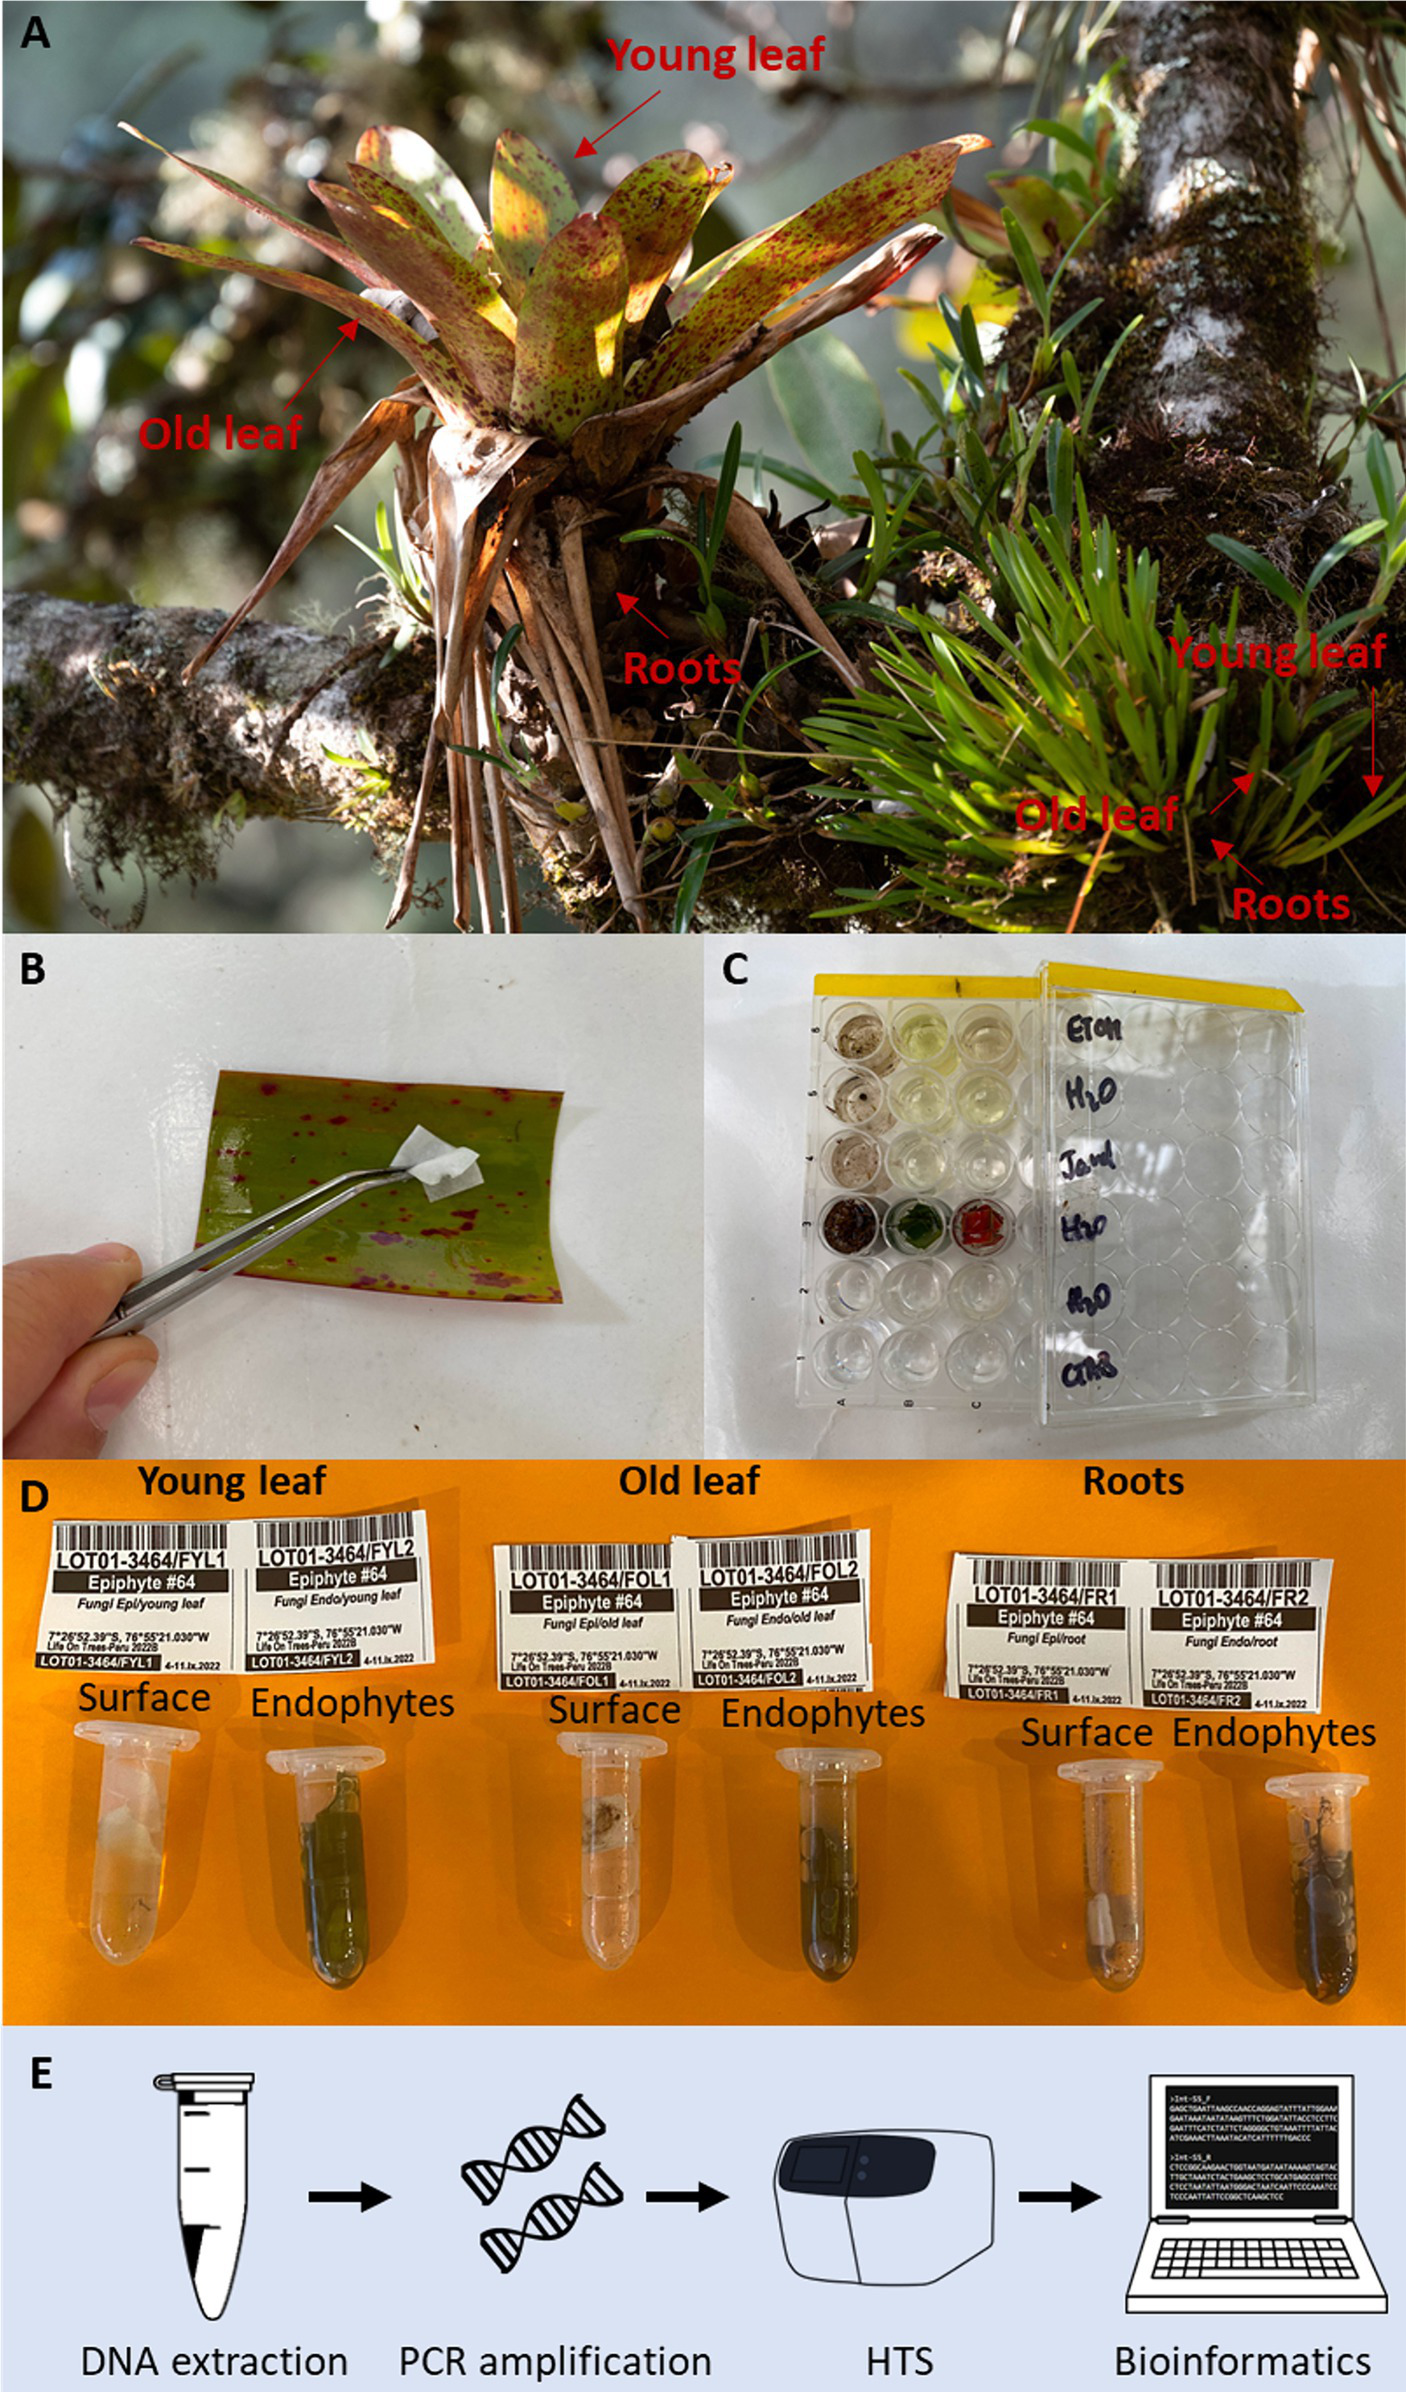
\includegraphics[width=\linewidth]{Figures/sampling_protocol.png}
    \end{minipage}
    \hfill
    \begin{minipage}[c]{0.54\textwidth}
        \caption[Procédure pour l'isolement des champignons de surface et endophytes chez les plantes épiphytes.]{Procédure pour l'isolement des champignons de surface et endophytes chez les plantes épiphytes.\\[0.3em]
        {\footnotesize (A) Pour chaque individu de plante épiphyte, une jeune feuille entièrement développée, une vieille feuille et différentes parties du système racinaire ont été échantillonnées. (B) L'échantillonnage des micromycètes de la surface de la feuille a été réalisé à l'aide d'un morceau de papier Whatman préalablement imbibé de tampon CTAB stérile. (C) Stérilisation de surface pour l'isolement des endophytes en trempant successivement les portions de tissus dans de l'éthanol à 70 \%, de l'eau stérile, de l'hypochlorite de sodium à 9 \%, puis en les lavant deux fois dans de l'eau stérile, et enfin en les immergeant dans un tampon CTAB stérile. (D) La conservation de l'ADN a été effectuée dans des tubes Eppendorf stériles avec du tampon CTAB. (E) Flux de travail du métabarcoding de l'ADN. Crédits images : (A) Charlie Delhumeau, (B--D) CL. \citep{leponce2024unveiling}}}
        \label{fig:ma_figure}
    \end{minipage}
\end{figure}

Les trois arbres étudiés dans le projet LOT s’échelonnent le long d’un gradient altitudinal dans les Andes péruviennes. Cette configuration offre un terrain d’exploration unique pour saisir l’impact de l’altitude et des conditions locales sur la diversité fongique. Le premier site, LOT1, se situe à environ 400 mètres d’altitude, en pleine Amazonie. Ici, la chaleur et l’humidité règnent en maîtres. Plus haut, à 800 mètres, LOT2 occupe une zone de transition, à la frontière entre la forêt tropicale de plaine et les premiers contreforts montagneux. Enfin, LOT3 culmine à 2500 mètres, au cœur de la forêt de nuage andine. Ce dernier site se distingue par des températures plus fraîches, une humidité persistante et une lumière tamisée par la brume.

Tous ces sites sont rattachés à la station biologique de Wayqecha, dans la région de Cusco, gérée par l’ONG Amazon Conservation. Ce choix n’est pas anodin : il permet de s’appuyer sur un suivi écologique de longue durée et sur des infrastructures de recherche solides. Les arbres sélectionnés appartiennent à différentes espèces. LOT1 est un \textit{Dussia tessmannii} (Fabaceae), LOT2 un \textit{Ficus americana subsp. andicola} (Moraceae) et LOT3 un \textit{Brosimum cf. utile} (Moraceae). Ils servent de support pour inventorier la biodiversité associée à un seul hôte. En comparant à la fois différents sites et divers microhabitats au sein de chaque arbre, cette approche vise à mieux comprendre comment les gradients environnementaux et les caractéristiques propres à chaque arbre influencent la structuration des communautés fongiques chez les plantes épiphytes vasculaires tropicales.

L’échantillonnage suivi dans ce travail reprend le protocole décrit par \citet{leponce2024unveiling}. Les communautés fongiques ont été étudiées à partir de plantes épiphytes vasculaires déjà collectées. Pour chaque individu, trois compartiments ont été ciblés afin de représenter différents microhabitats de la plante hôte : une jeune feuille entièrement développée, une vieille feuille et plusieurs portions du système racinaire.

Deux fractions fongiques ont ensuite été distinguées. Les champignons présents à la surface des feuilles ont été prélevés par frottis à l’aide d’un papier Whatman stérile imbibé de tampon CTAB. Les endophytes, eux, ont été isolés après une stérilisation de surface des tissus végétaux. Celle-ci reposait sur une succession de bains d’éthanol, d’eau stérile et d'hypochlorite de sodium, puis sur plusieurs rinçages avant la conservation des échantillons dans le tampon CTAB. Cette étape était essentielle, car elle permettait de distinguer les champignons vivant à la surface des organes de ceux présents à l’intérieur des tissus.

La caractérisation des communautés fongiques a ensuite reposé sur une approche de métabarcoding haut débit ciblant la région ITS (\textit{Internal Transcribed Spacer}), couramment utilisée comme marqueur de référence pour l’étude de la diversité fongique. Après amplification par PCR, les produits obtenus ont été séquencés sur une plateforme Illumina MiSeq. Le traitement bioinformatique a compris plusieurs étapes successives : démultiplexage des lectures, contrôle qualité, suppression des séquences de faible qualité et des chimères, puis regroupement en unités taxonomiques opérationnelles (OTUs). Une assignation taxonomique a ensuite été réalisée à l’aide de bases de référence adaptées aux champignons. Au terme de cette chaîne d’analyse, une table de contingence recensant le nombre de séquences par échantillon a été obtenue. C’est sur cette base qu’ont été menées l’ensemble des analyses de diversité et de composition présentées ici \citep{leponce2024unveiling}.


\subsection{Analyses de diversité}

Pour comparer la diversité alpha, nous avons utilisé les nombres de Hill, suivant l’approche développée par \citet{chao2014rarefaction}. Cette méthode permet de représenter à la fois la raréfaction, c’est-à-dire l’interpolation, et l’extrapolation des courbes de diversité. Trois ordres ont été retenus. Le premier, \(q=0\), correspond à la richesse spécifique. Le second, \(q=1\), traduit le nombre effectif d’espèces associé à l’indice de Shannon. Enfin, \(q=2\) repose sur l’indice de Simpson et donne davantage de poids aux taxons dominants. Ces différents indices ont ensuite été comparés entre les microhabitats de la plante hôte — jeunes feuilles, vieilles feuilles et racines — ainsi qu’entre les trois sites d’échantillonnage (LOT1, LOT2 et LOT3).

Les courbes ont été générées sous \texttt{R} avec le package \texttt{iNEXT.3D} \citep{chao2021measuring}. Des intervalles de confiance à 95\,\% ont été estimés par bootstrap à partir de 50 réplicats. Ce cadre d’analyse est particulièrement utile lorsque l’effort d’échantillonnage varie d’une catégorie à l’autre, car il permet de comparer les niveaux de diversité sur une base standardisée.

Nous avons également calculé l’équitabilité à l’aide de l’indice de Pielou, défini par :

\[
J = \frac{H'}{\ln(S)}
\]

où \(H'\) désigne l’indice de Shannon et \(S\) la richesse spécifique. Cet indice permet d’évaluer dans quelle mesure les abondances sont réparties de façon homogène au sein des communautés fongiques.

\subsection{Partage des OTUs et abondances relatives}
Le partage des OTUs entre microhabitats a été étudié à l’aide de diagrammes UpSet \citep{lex2014upset}. Ce type de représentation est particulièrement utile pour comparer plusieurs ensembles à la fois. Il reste aussi plus lisible qu’un diagramme de Venn dès que le nombre de catégories devient important. Il permet ainsi de repérer les OTUs communs à plusieurs compartiments de la plante, mais aussi ceux qui semblent propres à un microhabitat donné. Les graphiques ont été produits sous \texttt{R} avec le package \texttt{UpSetR} \citep{conway2017upsetr}.

Pour compléter cette approche, les taxons les plus abondants dans chaque microhabitat ont été résumés dans un tableau de chaleur. Les données ont été exprimées en abondances relatives, puis transformées en scores Z (centrées et réduites par microhabitat), afin de comparer les profils malgré les différences de profondeur de séquençage. Cette représentation permet de visualiser rapidement les OTUs dominants et de mieux faire ressortir les variations de composition entre jeunes feuilles, vieilles feuilles et racines. Le tableau a été construit à partir des OTUs présents dans au moins 5\% des échantillons de chaque microhabitat, avec le package \texttt{pheatmap} sous \texttt{R} \citep{kolde2019pheatmap}. Le score Z est défini comme la différence entre la valeur observée et la moyenne, divisée par l'écart-type \citep{altman1991practical}.

Ces deux approches se complètent. Les diagrammes UpSet décrivent le degré de partage des OTUs entre habitats, tandis que le tableau de chaleur met en avant les taxons dominants qui contribuent le plus aux différences observées entre compartiments.

\subsection{Analyses de similarités}

Pour étudier les différences de composition entre communautés fongiques, nous avons analysé la diversité bêta à partir d’une matrice de dissimilarité de Bray--Curtis calculée sur les abondances relatives des OTUs \citep{bray1957ordination}. Cette mesure est couramment utilisée pour les données de communautés, car elle intègre l’information d’abondance tout en restant peu sensible aux doubles absences.

La structure des assemblages a ensuite été explorée par une ordination NMDS (\textit{Non-metric Multidimensional Scaling}), réalisée sous \texttt{R} \citep{kruskal1964nonmetric,minchin1987evaluation}. L’objectif de cette approche est de projeter les échantillons dans un espace de faible dimension, de façon à restituer au mieux les relations de similarité observées entre eux. La qualité de cette représentation a été évaluée à l’aide de la valeur de stress. Des valeurs inférieures à 0{,}2 sont considérées comme suffisamment fiables pour une interprétation écologique \citep{kruskal1964nonmetric}.

Enfin, les différences de composition entre groupes ont été testées par PERMANOVA (\textit{Permutational Multivariate Analysis of Variance}) avec la fonction \texttt{adonis2} du package \texttt{vegan} \citep{anderson2001new} à 999 permutations. Selon le jeu de données considéré, les effets du site (LOT1, LOT2, LOT3) et du microhabitat (jeunes feuilles, vieilles feuilles, racines) ont été examinés séparément. La significativité a été évaluée par permutations, et les résultats sont présentés sous la forme du \(R^2\), de la statistique pseudo-\(F\) de Fisher et de la valeur de \(p\).

\subsection{Spécialisation des niches fongiques}

L’amplitude de niche des OTUs a été évaluée à partir de l’indice de Levins \citep{levins1968evolution}. Cet indice permet d’apprécier dans quelle mesure un taxon est réparti entre plusieurs microhabitats. En pratique, il aide à distinguer des OTUs plutôt généralistes, présents dans différents compartiments de la plante, de taxons plus spécialisés, associés à un nombre plus limité d’habitats.

Pour chaque OTU \(j\), l’indice brut a été calculé de la manière suivante :

\[
B_j = \frac{1}{\sum_{i=1}^{n} p_{ij}^{2}}
\]

dans laquelle \(p_{ij}\) correspond à la proportion relative de l’OTU \(j\) dans le microhabitat \(i\), et \(n\) au nombre total de microhabitats pris en compte. Lorsque \(B_j\) est élevé, cela signifie que l’OTU est réparti de façon plus homogène entre les habitats considérés et présente donc une niche plus large.

Pour rendre les comparaisons entre taxons plus directes, une version standardisée de cet indice a aussi été utilisée :

\[
B_{A} = \frac{B_j - 1}{n - 1}
\]

Cette transformation ramène les valeurs entre 0 et 1. Des valeurs faibles traduisent une forte spécialisation, tandis que des valeurs plus élevées indiquent au contraire une occupation plus régulière des différents microhabitats. Afin d’éviter que les taxons rares ne brouillent les tendances générales, l’analyse a été restreinte aux OTUs les plus abondants. Cela permet de mieux faire ressortir les grands patrons de spécialisation au sein des communautés fongiques associées aux plantes épiphytes.




\section{Résultats}

\subsection{Analyses de diversité Alpha}

\begin{figure}[!h]
    \centering
    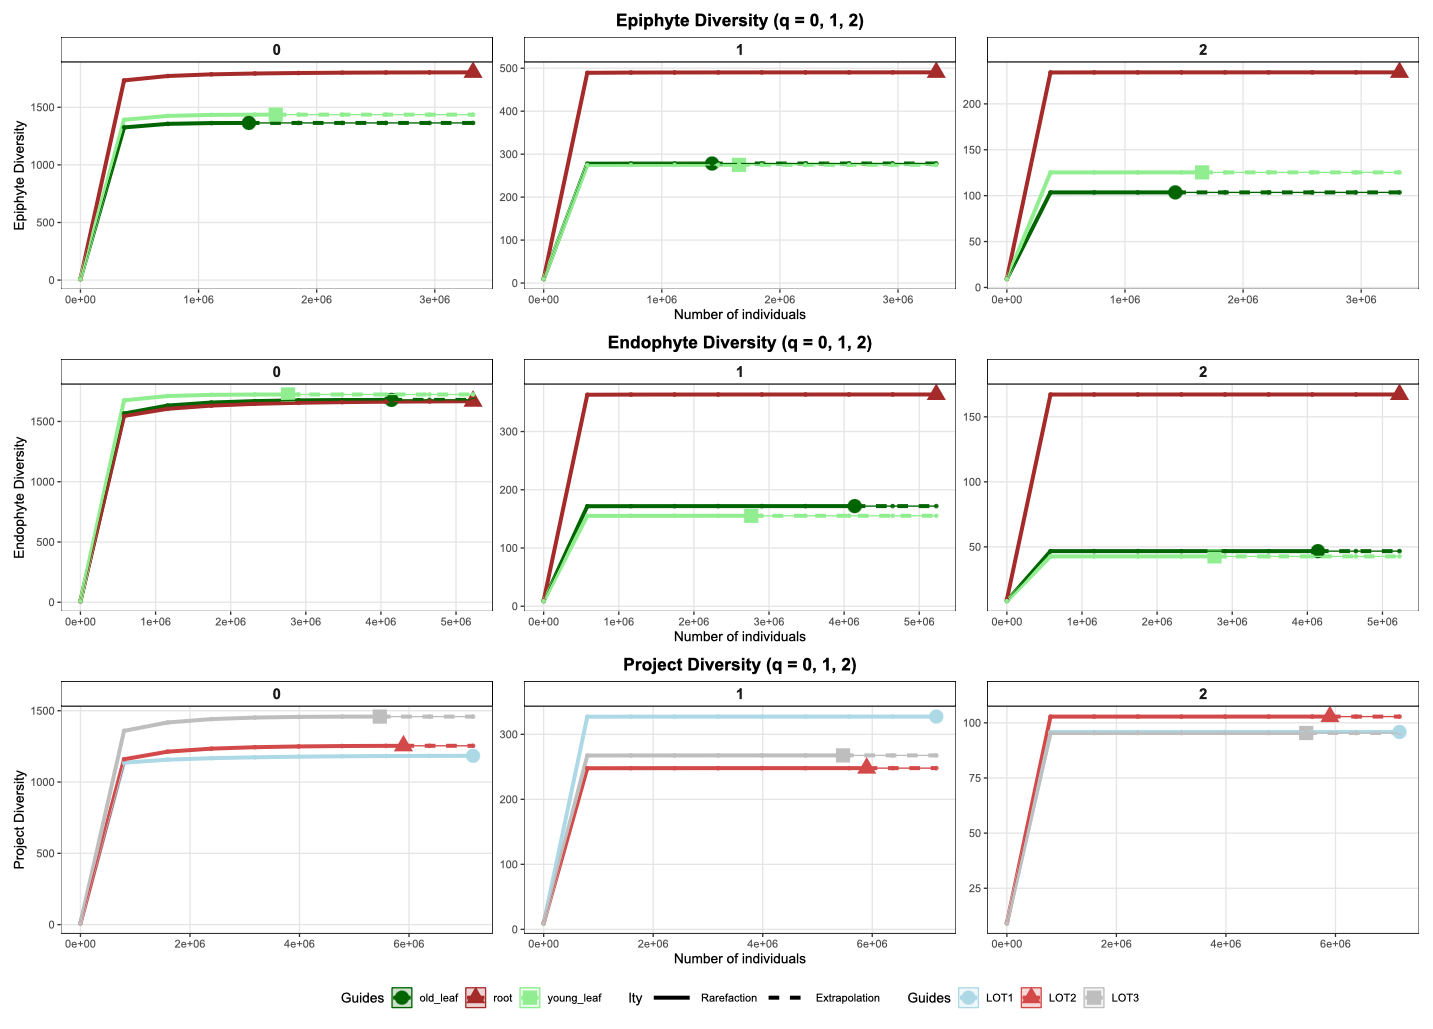
\includegraphics[width=1\textwidth]{Figures/rarefaction_alpha_div.png}
    \caption{Courbes de raréfaction et d'extrapolation pour la diversité alpha
    (q=0 : richesse spécifique, q=1 : diversité de Shannon exponentielle et
    q=2 : diversité de Simpson inverse) des communautés fongiques associées aux
    plantes épiphytes. Les courbes sont présentées pour différents organes
    (feuilles jeunes, feuilles vieilles, racines) ou différents sites
    (LOT1, LOT2 ou LOT3). Les intervalles de confiance à 95\% sont indiqués
    par des zones ombrées.}
    \label{fig:inext}
    \end{figure}

    Les courbes de raréfaction et d’extrapolation (figure \ref{fig:inext}) révèlent des contrastes marqués de diversité alpha, aussi bien entre microhabitats qu’entre sites. On remarque que les courbes pour les indices \(q=0\), \(q=1\) et \(q=2\) atteignent rapidement un plateau, ce qui suggère que l’échantillonnage a permis de bien cerner la diversité des taxons les plus fréquents et dominants. 

    Si l’on compare les différents organes, les racines se distinguent nettement par leurs valeurs de diversité, systématiquement plus élevées que celles des feuilles pour les indices de Shannon et de Simpson (voir tableau \ref{tab:diversite_alpha}). Chez les épiphytes de surface, elles affichent la plus forte richesse (\(2603.267 \pm 4.366\)), mais aussi les diversités de Shannon (\(584.089 \pm 0.442\)) et de Simpson (\(255.381 \pm 0.287\)) les plus importantes. Chez les endophytes, la richesse spécifique (\(q=0\)) des racines (\(2422.284 \pm 6.803\)) est légèrement inférieure à celle des jeunes feuilles (\(2466.674 \pm 5.309\)), mais les racines présentent des niveaux de diversité bien supérieurs pour \(q=1\) (\(413.761 \pm 0.228\)) et \(q=2\) (\(176.767 \pm 0.162\)). À l’inverse, les feuilles, surtout chez les endophytes, hébergent des communautés moins équilibrées, dominées par un petit nombre d’OTUs.

    Les différences entre feuilles jeunes et vieilles varient selon la fraction fongique considérée. Chez les épiphytes de surface, les vieilles feuilles montrent une richesse légèrement inférieure à celle des jeunes feuilles, mais une diversité de Shannon et de Simpson un peu plus élevée. Cela laisse penser que la distribution des abondances y est plus homogène. Pour les endophytes, les feuilles jeunes et vieilles présentent des richesses proches (\(\sim 2400{-}2460\) OTUs), mais les indices \(q=1\) et \(q=2\) restent faibles, ce qui traduit une forte dominance de quelques taxons. Les indices d’équitabilité confirment cette tendance : ils sont particulièrement bas dans les feuilles endophytiques (\(J = 0.07\) à \(0.08\)), alors qu’ils atteignent des valeurs plus élevées dans les racines (\(J = 0.17\) à \(0.22\)).

    Du côté des sites, c’est à LOT3 que la richesse spécifique atteint son maximum (\(2031 \pm 5.601\)), tandis que LOT1 se distingue par la plus forte diversité de Shannon (\(381.82 \pm 0.281\)) et la meilleure équitabilité (\(J = 0.23\)). LOT2, quant à lui, présente une richesse intermédiaire et la diversité de Simpson la plus élevée (\(110.127 \pm 0.152\)). Toutefois, les écarts entre sites restent moins prononcés que ceux observés entre organes. Globalement, ces résultats montrent que le microhabitat, et en particulier l’opposition racines/feuilles, façonne plus fortement la diversité alpha des communautés fongiques que la localisation géographique du site.
    \begin{table}[!h]
        \centering

            \centering
            {\fontsize{8}{9.6}\selectfont
            \renewcommand{\arraystretch}{1.25}
            \setlength{\tabcolsep}{15pt}
            \resizebox{\textwidth}{!}{%
            \begin{tabular}{llllll}
                \hline
                \textbf{Position} & \textbf{Organes} & \textbf{Richesse (q0)} & \textbf{Shannon (q1)} & \textbf{Simpson (q2)} & \textbf{Équitabilité} \\
                \hline
                \multicolumn{6}{l}{\textbf{Diversité par organes et position}} \\
                Epiphytes  & Old leaf   & $1903.132 \pm 4.092$ & $335.264 \pm 0.452$ & $113.957 \pm 0.297$ & 0.18 \\[0.2em]
                           & Root       & $2603.267 \pm 4.366$ & $584.089 \pm 0.442$ & $255.381 \pm 0.287$ & 0.22 \\[0.2em]
                           & Young leaf & $2018.329 \pm 5.493$ & $324.232 \pm 0.387$ & $135.603 \pm 0.229$ & 0.16 \\[0.3em]
                Endophytes & Old leaf   & $2415.849 \pm 6.878$ & $199.032 \pm 0.203$ & $49.380 \pm 0.073$  & 0.08 \\[0.2em]
                           & Root       & $2422.284 \pm 6.803$ & $413.761 \pm 0.228$ & $176.767 \pm 0.162$ & 0.17 \\[0.2em]
                           & Young leaf & $2466.674 \pm 5.309$ & $177.815 \pm 0.221$ & $44.826 \pm 0.078$  & 0.07 \\
                \multicolumn{6}{l}{\textbf{Diversité par projets}} \\
                Projets    & LOT1       & $1680.161 \pm 4.884$ & $381.82 \pm 0.281$  & $102.611 \pm 0.147$ & 0.23 \\[0.2em]
                           & LOT2       & $1753.821 \pm 5.547$ & $290.496 \pm 0.232$ & $110.127 \pm 0.152$ & 0.17 \\[0.2em]
                           & LOT3       & $2031 \pm 5.601$     & $306.332 \pm 0.195$ & $101.155 \pm 0.114$ & 0.15 \\
                \hline
            \end{tabular}%
            }}
\caption{Diversité alpha des communautés fongiques selon la catégorie et l'assemblage.}
            \label{tab:diversite_alpha}

    \end{table}


\subsection{Partage des OTUs et abondances relatives}

\begin{figure}[!h]
    \centering
    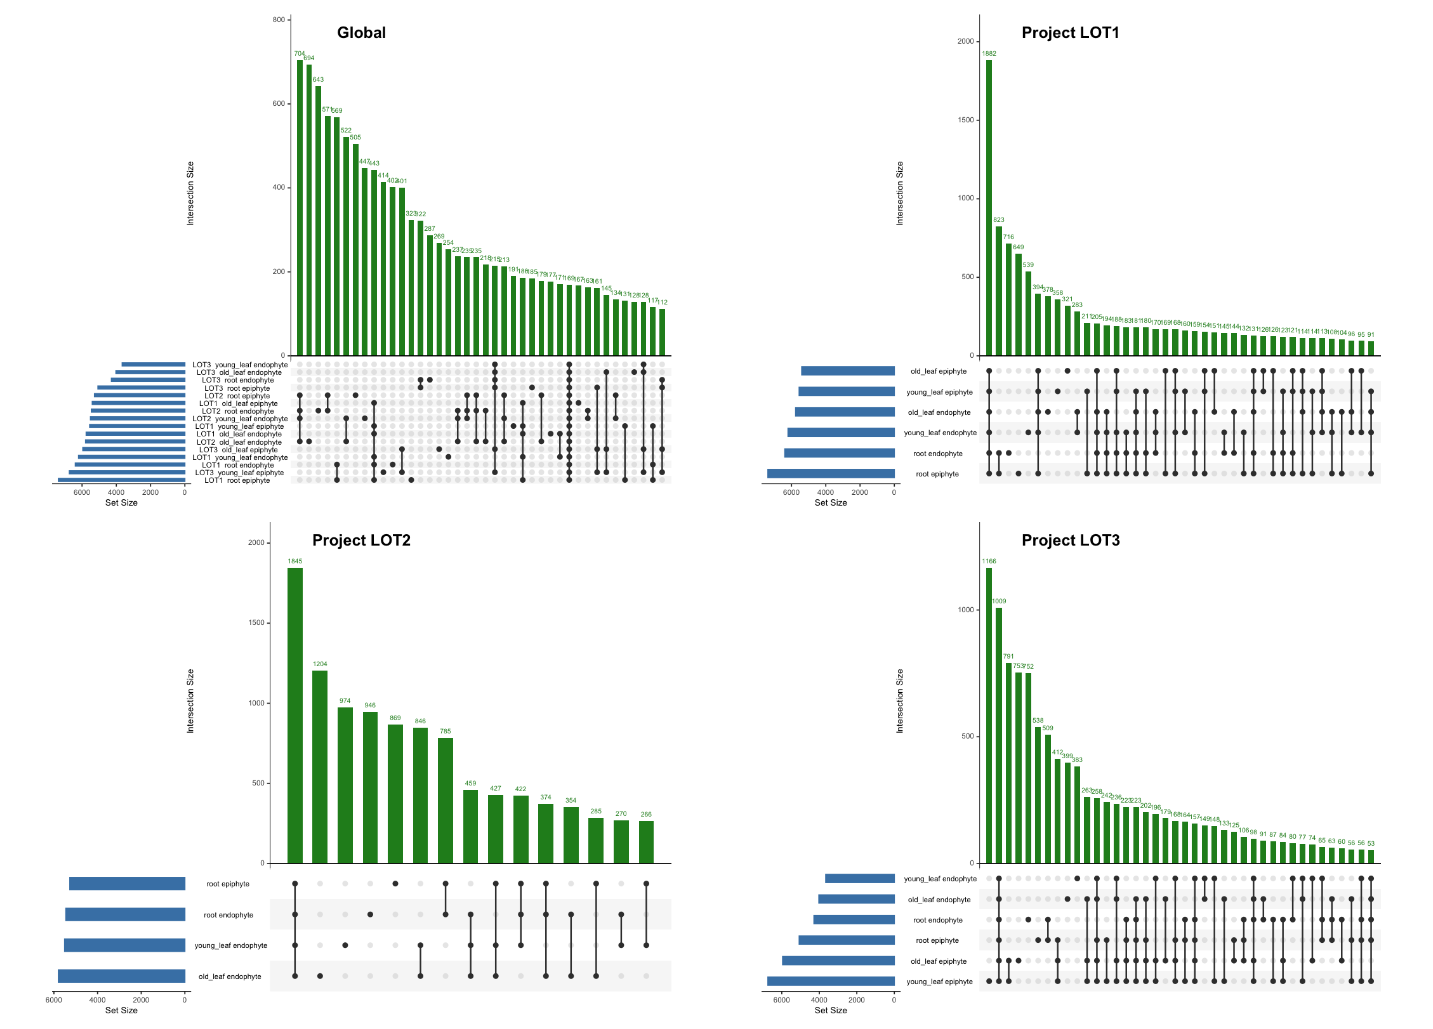
\includegraphics[width=1\textwidth]{Figures/upset_plots.png}
    \caption{Diagrammes UpSet pour les OTUs partagés entre les microhabitats.}
    \label{fig:upset}
\end{figure}

Les diagrammes UpSet (figure \ref{fig:upset}) illustrent la répartition des OTUs entre les différents microhabitats. On observe qu’un noyau d’OTUs est partagé par plusieurs compartiments, mais une grande partie de la diversité reste propre à chaque organe. Les racines, en particulier, se démarquent par un nombre élevé d’OTUs exclusifs. Cela traduit une composition fongique originale, distincte de celle des feuilles. À l’opposé, les feuilles jeunes et vieilles partagent davantage leurs communautés, ce qui suggère une proximité écologique entre ces deux types de tissus.

Ce constat rejoint les résultats de diversité alpha, qui montraient déjà une richesse particulièrement élevée dans les racines. Il semble donc que ce microhabitat soit à la fois un refuge pour des taxons spécialisés et un point de rencontre pour des espèces plus généralistes. Les feuilles, quant à elles, hébergent des assemblages plus proches, probablement en raison de conditions environnementales et physiologiques similaires.

En résumé, la distribution des OTUs fongiques apparaît fortement structurée par le microhabitat. Les différences entre organes souterrains et aériens sont nettes, et le rôle du compartiment racinaire comme réservoir de diversité se confirme à travers ces analyses.

\begin{figure}[!h]
    \centering
    \begin{minipage}[c]{0.62\textwidth}
        \centering
        \includegraphics[width=\linewidth]{Figures/heatmap_orders.png}
    \end{minipage}
    \hfill
    \begin{minipage}[c]{0.33\textwidth}
        \caption{Tableau des OTUs les plus abondants dans chaque microhabitat.}
        \label{fig:abondances}
    \end{minipage}
\end{figure}



Le tableau de chaleur des OTUs les plus abondants (figure \ref{fig:abondances}) illustre clairement à quel point la composition des communautés varie d’un microhabitat à l’autre. Les racines, par exemple, se démarquent nettement : elles hébergent un ensemble d’OTUs dominants qui diffèrent en grande partie de ceux retrouvés dans les feuilles. Ce contraste souligne la forte structuration des assemblages fongiques selon l’organe étudié. À l’inverse, les feuilles jeunes et vieilles affichent des profils d’abondance plus similaires. On y retrouve plusieurs OTUs dominants communs, même si leur abondance relative varie parfois sensiblement d’un compartiment à l’autre.


On remarque aussi que la distribution des taxons dominants n’est pas homogène. Certains OTUs semblent presque exclusifs à un seul microhabitat, ce qui suggère une affinité particulière pour des conditions locales spécifiques. D’autres, au contraire, sont présents dans plusieurs compartiments, mais leur importance relative fluctue fortement selon l’organe. Cette organisation montre que les différences entre organes ne reposent pas uniquement sur la présence ou l’absence de certains taxons, mais aussi sur des changements dans la hiérarchie d’abondance parmi les OTUs partagés.

Dans l’ensemble, ces observations rejoignent les résultats des diagrammes UpSet et des analyses de diversité alpha. Les racines apparaissent comme un réservoir de diversité original, tandis que les feuilles partagent davantage leurs taxons dominants. Ainsi, le microhabitat au sein de la plante hôte s’impose comme un facteur clé, à la fois pour la composition et pour la structure d’abondance des communautés fongiques.

\subsection{Analyses de similarités}
\begin{figure}[!h]
    \centering
    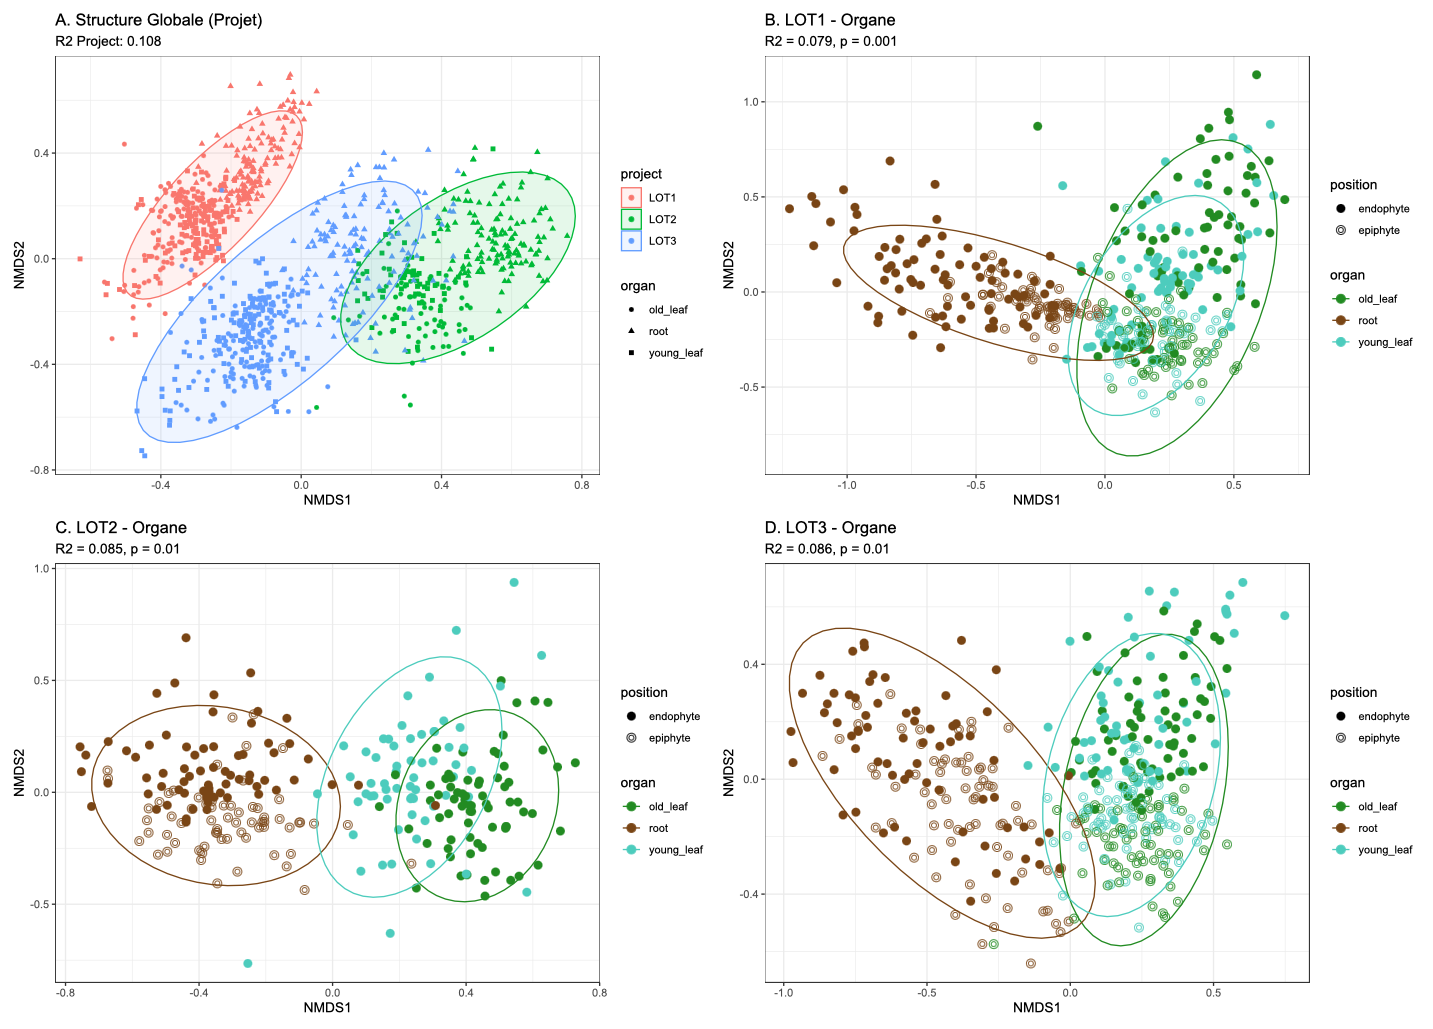
\includegraphics[width=1\textwidth]{Figures/NMDS.png}
    \caption{Ordination NMDS des communautés fongiques associées aux plantes épiphytes.}
    \label{fig:nmds}
\end{figure}

L’ordination NMDS (figure \ref{fig:nmds}) révèle une structuration nette des communautés fongiques, à la fois selon le site d’échantillonnage et le microhabitat (voir tableau \ref{tab:permanova_nmds}). À l’échelle globale (panel A), on observe que les échantillons tendent à se regrouper en fonction du projet LOT, ce qui traduit un effet du site sur la composition des assemblages. La PERMANOVA confirme cette tendance (\(R^2 = 0.108\), pseudo-\(F = 69.483\), \(p = 0.010\)), même si une part importante de la variation reste partagée entre les différents sites.

Lorsqu’on examine chaque projet séparément (panels B à D), la structuration selon l’organe devient également très marquée. Dans les trois sites, les racines forment un groupe distinct, bien séparé des feuilles, tandis que les feuilles jeunes et vieilles présentent un recouvrement plus important. Les tests de PERMANOVA montrent un effet significatif de l’organe dans le LOT1 (\(R^2 = 0.079\), \(F = 17.802\), \(p = 0.001\)), LOT2 (\(R^2 = 0.085\), \(F = 12.716\), \(p = 0.010\)) et LOT3 (\(R^2 = 0.086\), \(F = 19.752\), \(p = 0.010\)).

Les valeurs de stress des ordinations, comprises entre \(0.136\) et \(0.150\), restent bien en dessous du seuil de 0{,}2. Cela garantit une représentation fidèle des relations de dissimilarité entre échantillons. En résumé, ces analyses montrent que la composition des communautés fongiques varie non seulement entre les sites andins, mais aussi, et surtout, entre les différents organes de la plante hôte. L’effet du microhabitat apparaît ainsi particulièrement déterminant dans la structuration de ces assemblages.
\begin{table}[!h]
    \centering
    \caption{Résultats des analyses de structure des communautés fongiques par NMDS et PERMANOVA selon les panels présentés en figure \ref{fig:nmds}.}
    \label{tab:permanova_nmds}
    \vspace{0.5cm}

    \renewcommand{\arraystretch}{1.2}
    \setlength{\tabcolsep}{8pt}
    \resizebox{\textwidth}{!}{%
    \begin{tabular}{llllllllll}
        \hline
        \textbf{Panel} & \textbf{Analyse} & \textbf{Effet testé} & \textbf{Échantillons} & \textbf{Df} & \textbf{R\textsuperscript{2}} & \textbf{F} & \textbf{p-value} & \textbf{Significativité} & \textbf{Stress NMDS} \\
        \hline
        A & Structure globale (Projet) & Projet & 1075 & 2 & 0.108 & 69.483 & 0.001 & ** & 0.136 \\
        B & LOT1 -- Organe             & Organe & 402  & 2 & 0.079 & 17.802 & 0.001 & ** & 0.150 \\
        C & LOT2 -- Organe             & Organe & 267  & 2 & 0.085 & 12.716 & 0.001 & ** & 0.148 \\
        D & LOT3 -- Organe             & Organe & 406  & 2 & 0.086 & 19.752 & 0.001 & ** & 0.149 \\
        \hline
        \end{tabular}%
    }
\end{table}


\subsection{Spécialisation des niches fongiques}



\begin{figure}[!h]
    \centering
    \begin{minipage}[c]{0.68\textwidth}
        \centering
        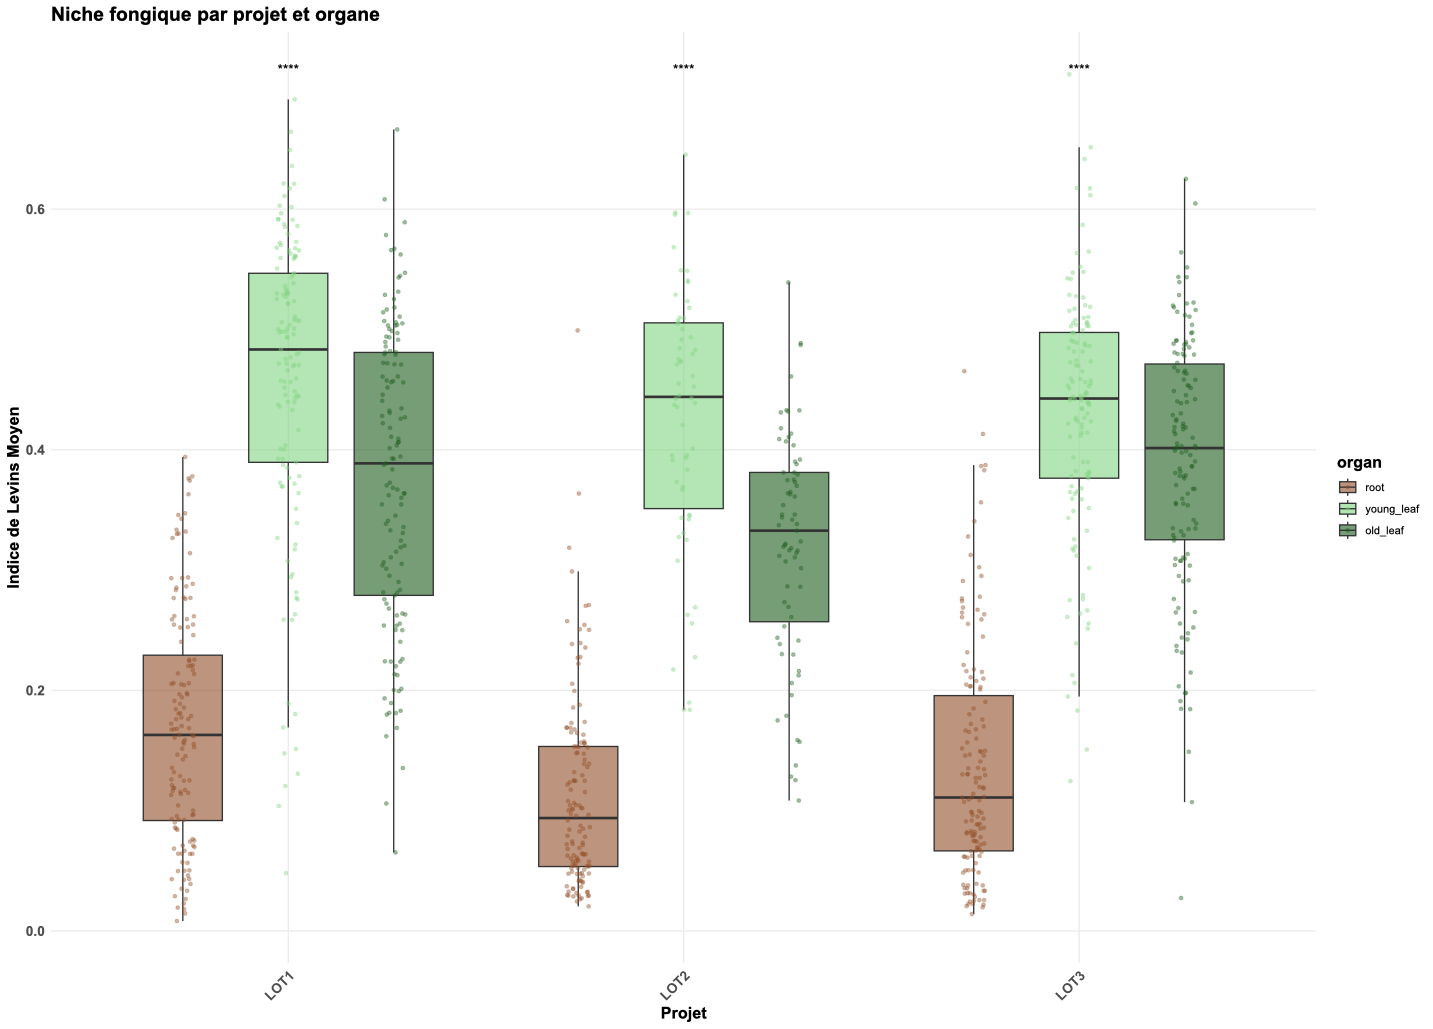
\includegraphics[width=\linewidth]{Figures/niches_de_levins.png}
    \end{minipage}
    \hfill
    \begin{minipage}[c]{0.28\textwidth}
        \caption{Indice de Levins pour les OTUs les plus abondants dans chaque microhabitat.}
        \label{fig:niches_levins}
    \end{minipage}
\end{figure}

L’examen des valeurs de l’indice de Levins (figure \ref{fig:niches_levins}) met en lumière une grande diversité d’amplitudes de niche parmi les OTUs dominants. Beaucoup de taxons affichent des scores faibles à intermédiaires, ce qui traduit une répartition inégale entre les différents microhabitats et suggère une certaine spécialisation. À l’opposé, quelques OTUs se distinguent par des valeurs nettement plus élevées, caractéristiques d’un comportement généraliste et d’une présence plus équilibrée dans plusieurs compartiments de la plante.

Les OTUs dominants retrouvés dans les racines illustrent particulièrement bien ce phénomène de spécialisation. Plusieurs d’entre eux semblent presque exclusivement associés à ce microhabitat, confirmant ainsi que les racines abritent un ensemble original de champignons adaptés à des conditions spécifiques. Ce constat fait écho aux résultats précédents, qui montraient déjà une richesse élevée et une composition singulière dans ce compartiment.

Du côté des feuilles, qu’elles soient jeunes ou vieilles, les OTUs dominants présentent le plus souvent des amplitudes de niche intermédiaires. Cela laisse penser que ces deux types de tissus partagent une partie de leur cortège fongique, sans pour autant être identiques. Les conditions écologiques des feuilles, bien que proches, permettent à certains taxons de s’installer dans les deux compartiments, tandis que d’autres restent plus fidèles à un stade foliaire particulier.

En somme, l’analyse de l’indice de Levins met en évidence une organisation non aléatoire des communautés fongiques au sein de la plante hôte. On observe une coexistence de spécialistes, principalement cantonnés à un microhabitat, et de généralistes capables d’occuper plusieurs compartiments. Ce schéma confirme le rôle central du microhabitat comme filtre écologique dans l’assemblage des communautés fongiques associées aux plantes épiphytes.


\section{Discussion}




\singlespacing
\newpage
\listoffigures
\listoftables
\newpage

\bibliography{BIBLIO_Stage_LOT_CRBE.bib}
\bibliographystyle{apalike}

\end{document}